% The delusional spiral, and where to break it.
% ---------------------------------------------------------------------------
% style.tex --- shared preamble for every figure in book/figures/tikz/
%
% One style for all figures: Latin Modern, thin black lines, a light grey
% fill, and one accent colour used only to mark what is untrusted or wrong.
% Build with scripts/build_figures.sh; see book/figures/README.md.
% ---------------------------------------------------------------------------
\documentclass[tikz,border=6pt]{standalone}
\usepackage[T1]{fontenc}
\usepackage{lmodern}
\usetikzlibrary{arrows.meta,positioning,shapes.geometric,calc,fit,backgrounds}

\hyphenpenalty=10000   % short lines in boxes: ragged, never hyphenated

\definecolor{lightgrey}{gray}{0.92}
\definecolor{accent}{HTML}{9B2D20}

\tikzset{
  every picture/.style={
    line width=0.6pt,
    font=\small,
    >={Stealth[length=5pt,width=4pt]},
    node distance=14pt and 24pt,
  },
  % shapes
  box/.style={draw, rectangle, inner xsep=8pt, inner ysep=5pt,
              minimum height=22pt, align=center},
  grey/.style={box, fill=lightgrey},
  rounded/.style={box, rounded corners=9pt},
  decision/.style={draw, diamond, aspect=2.4, inner sep=1.5pt, align=center},
  group/.style={draw, dashed, rounded corners=5pt, inner sep=7pt},
  % text
  tag/.style={font=\footnotesize, align=center, inner sep=2pt},
  note/.style={font=\footnotesize\itshape, align=center, inner sep=2pt},
  code/.style={font=\small\ttfamily},
  codetag/.style={font=\footnotesize\ttfamily, align=center, inner sep=2pt},
  title/.style={font=\small\scshape, align=center, inner sep=2pt},
  % lines
  arrow/.style={->},
  back/.style={->, dashed},
  thin/.style={line width=0.4pt, gray},
  % the one accent, for what is untrusted, wrong or missing
  bad/.style={accent},
  badbox/.style={box, draw=accent, text=accent},
}

\begin{document}
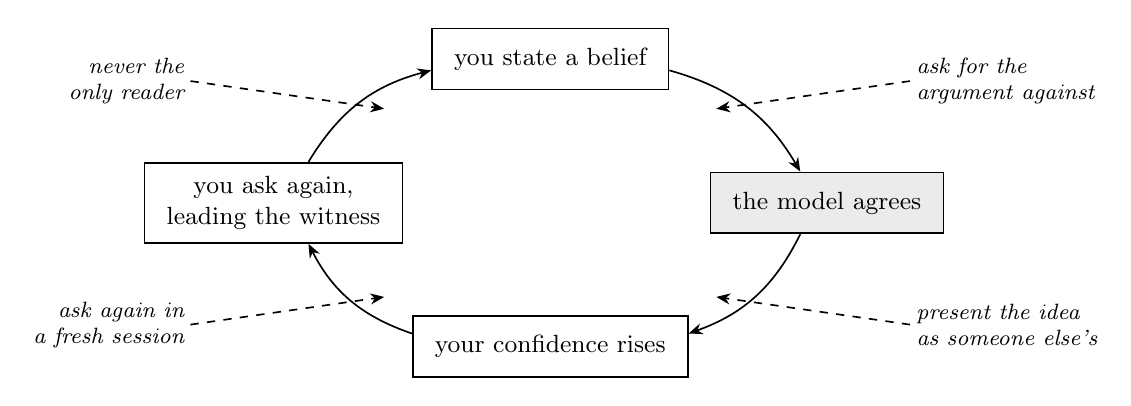
\begin{tikzpicture}
  \node[box] (a) at (0,52pt) {you state a belief};
  \node[grey] (b) at (100pt,0) {the model agrees};
  \node[box] (c) at (0,-52pt) {your confidence rises};
  \node[box] (d) at (-100pt,0) {you ask again,\\leading the witness};
  \draw[->] (a) to[bend left=22] (b);
  \draw[->] (b) to[bend left=22] (c);
  \draw[->] (c) to[bend left=22] (d);
  \draw[->] (d) to[bend left=22] (a);
  % where to cut
  \node[note, anchor=west, align=left] (n1) at (130pt,44pt) {ask for the\\argument against};
  \node[note, anchor=west, align=left] (n2) at (130pt,-44pt) {present the idea\\as someone else's};
  \node[note, anchor=east, align=right] (n3) at (-130pt,-44pt) {ask again in\\a fresh session};
  \node[note, anchor=east, align=right] (n4) at (-130pt,44pt) {never the\\only reader};
  \draw[back] (n1.west) -- ($(a)!0.5!(b)+(10pt,8pt)$);
  \draw[back] (n2.west) -- ($(b)!0.5!(c)+(10pt,-8pt)$);
  \draw[back] (n3.east) -- ($(c)!0.5!(d)+(-10pt,-8pt)$);
  \draw[back] (n4.east) -- ($(d)!0.5!(a)+(-10pt,8pt)$);
\end{tikzpicture}
\end{document}
